\section{Page Rank}
	\textbf{Page Rank} is a link analysis algorithm based on the Web graph (pages as nodes and hyper-links as edges), taking the rank value to indicate an importance of a particular page, which is defined recursively and	depends on the number of all pages that link to it (in-links).

	\subsection{The Simplest Model}
	The page in web can be regard as a node $A$ in a digraph $\mathcal G=(\mathcal V,\mathcal E)$. If the page $A$ have a hyper-link to page $B$, then there is a edge $A\rightarrow B$ in $\mathcal E$. For example, the web show in Figure \eqref{fig:fournodesweb} can be represented by a digraph $\mathcal G=(\mathcal V,\mathcal E)$ with
	\begin{gather*}
	\mathcal{V} =\{A,B,C,D\}\\
	\mathcal{E} =\{A\rightarrow B, A\rightarrow C,A\rightarrow D,B\rightarrow A,\\ B\rightarrow D,C\rightarrow A,D\rightarrow B,D\rightarrow C\}
	\end{gather*}
	\begin{figure}[h]
		\centering
		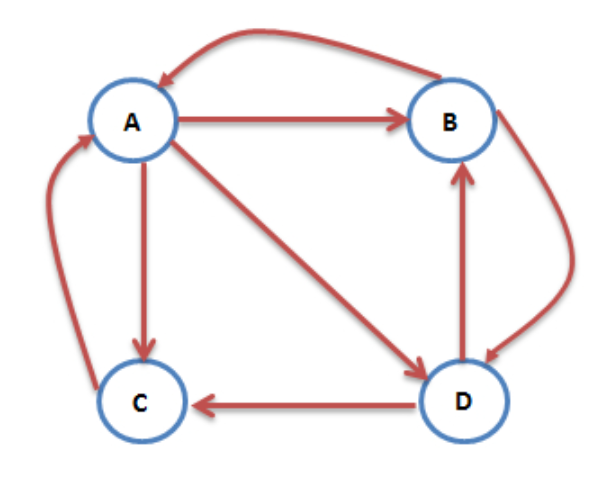
\includegraphics[width=0.7\linewidth]{fournodesweb}
		\caption{A web witch has 4 nodes}
		\label{fig:fournodesweb}
	\end{figure}
	
	Suppose there is a person Jack who is suffering the Internet, and at timing $t$, he is browsing page $A$. When he wants to leave page $A$, he will randomly click a hyper-link in page $A$ and go to browse next page and the possibility of clicking each page is the same. As an example in Figure \eqref{fig:fournodesweb}, each possibility from $A$ to $B,C,D$ are $\dfrac 13$. (If the page have no out-links, we can think it have a out-link to itself.) If we do that for each nodes, then we will have a transform matrix $M(\mathcal G)$. The transform matrix of the \eqref{fig:fournodesweb} is
	\begin{equation*}
		\begin{matrix}
		 to\backslash from&A&B&C&D\\
		A& &1/2 &1 &\\
		B&1/3 & & &1/2\\
		C&1/3 & & &1/2\\
		D&1/3 &1/2 & &
		\end{matrix}
	\end{equation*}
	i.e. 
	\begin{equation*}
	\mathbf M=\mathbf M(\mathcal{G})=
	\begin{pmatrix}
	 &1/2 &1 &\\
1/3 & & &1/2\\
1/3 & & &1/2\\
1/3 &1/2 & &
	\end{pmatrix}.
	\end{equation*}
	
	Now, we assume there are a large number of people, and at the timing $t=0$, each page has the same amount of people browsing it, i.e. for every page there are $\dfrac 1{|\mathcal V|}$ people browsing it at timing $t=0$. We use a vector $\mathbf v_0 =(\dfrac 1{|\mathcal V|},...,\dfrac 1{|\mathcal V|})^T$ to represent the initial state. 
	
	In the next timing $t=1$, every one randomly clicking a hyper-link in the page which he or she is browsing. Then the distribution of the people at $t=1$ is $$\mathbf v_1=\mathbf M\mathbf v_0.$$ By parity of reasoning, we can obtain the distribution of the people at $t=\mu$ is  $$\mathbf v_\mu=\mathbf M^\mu\mathbf v_0.$$
	
	We can regard this process is a Markov process, so the convergence of $\mathbf v_\mu$ is equivalent to the digraph $\mathcal G$ is \textbf{strongly connected}. So we have the following theorem:
	
	
	\begin{theorem}
		 $\mathbf v_\mu$ is convergent $\Leftrightarrow$ $\mathcal G$ is strongly connected
	\end{theorem}
	If we get the convergence result $\mathbf v_\infty$, the $i$th component $v_{\infty i}$ measures the importance of the $i$th page. Because the bigger $v_{\infty i}$ is, the more people will browse this page.
	Besides, by the theory of power method, we know if $\mathbf v_\mu$ is convergent, then the $\mathbf v_\infty$ is the corresponding eigenvector of the max eigenvalue of $\mathbf M$. 
	\subsection{More General Models}
	However the $\mathcal G$ of a real Internet web is impossible to be strongly connected, because there is always some pages have no out-links. Besides, if a page only have the out-link to itself, the result $\|\mathbf v_\infty\|$ may have no use value.
	
	Now we suppose Jack randomly click a hyper-link in the page with probability $\alpha$ or randomly input a new URL of a page with probability $1-\alpha$, so the iteration relation becomes:
	\begin{equation}\label{alpha}
	\mathbf v_{\mu+1}=(1-\alpha)\mathbf 1 +\alpha \mathbf M \mathbf v_\mu
	\end{equation}
	Because of $\|\mathbf v_0\|_1=1$ and the sum of each column of $\mathbf M$ is equal to 1, we can obtain $\|\mathbf v_\mu\|_1=1$ for any $\mu$. And the spectral radius of $\alpha \mathbf M$ is $$\rho(\alpha \mathbf M)=\alpha\rho(\mathbf M)\leq\alpha ||\mathbf M||_1=\alpha <1.$$ So the iteration \eqref{alpha} must be convergent, and $\mathbf v_\infty$ satisfy$$ 	\mathbf v_{\infty}=(1-\alpha)\mathbf 1 +\alpha \mathbf M \mathbf v_\infty.$$ 
	i.e.
	$$\mathbf v_\infty = (1-\alpha)(1-\alpha \mathbf M)^{-1}\mathbf 1 $$
